\section{Технологический раздел}

\subsection{Архитектура приложения}

Для приложения была выбрана клиент-серверная архитектура. Доступ к серверной части будет осуществляться с помощью API~\cite{api}. Для взаимодействия с базой данных будут использоваться коннекторы, предоставляющие интерфейс взаимодействия посредством языка программирования и, следовательно,  делать запросы из приложения. Приложение было разделено на компоненты: компонент доступа к данным, компонент бизнес-логики, компонент интерфейса. 

%Верхнеуровневое разбиение на компоненты представлено на рисунке~\ref{img:upper}

%\begin{figure}[!h]
%	\centering
%	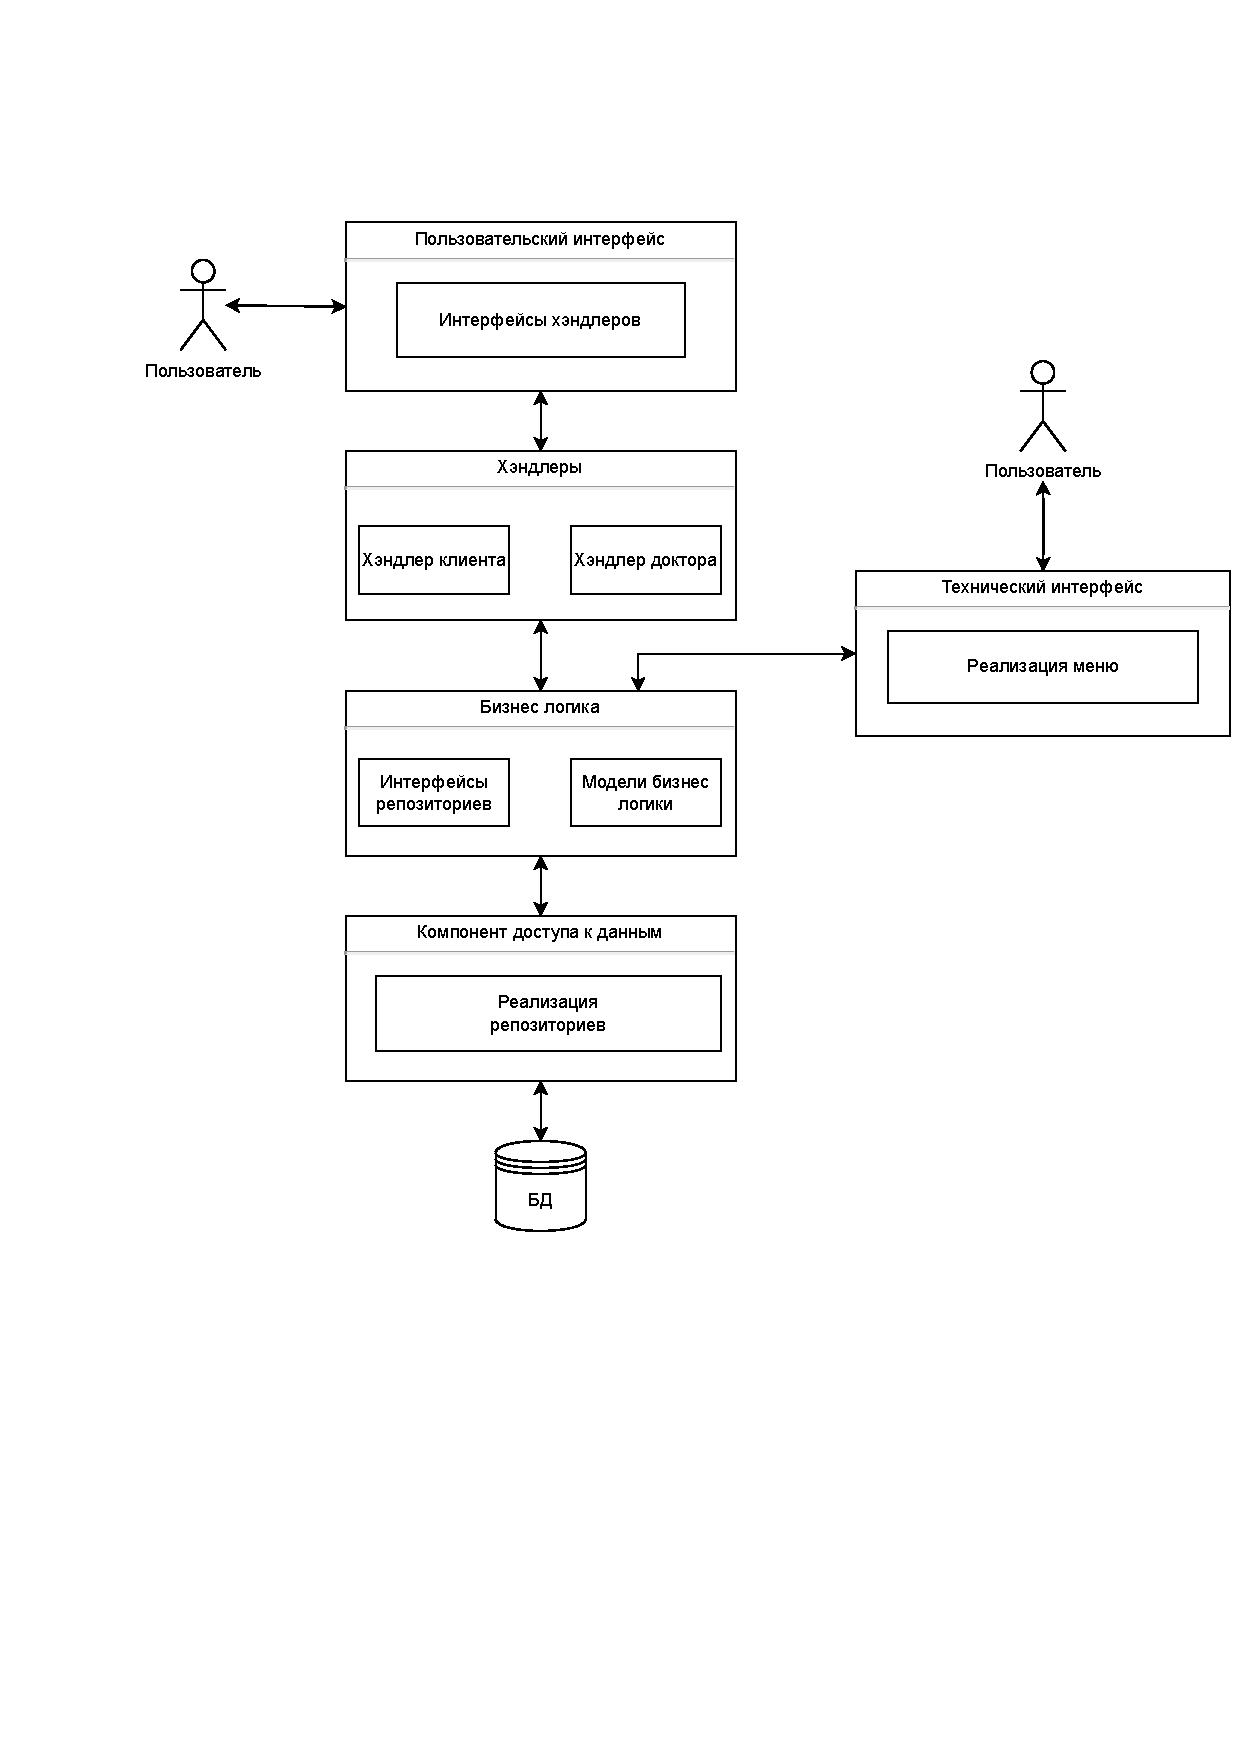
\includegraphics[width=\textwidth]{image/upper}
%	\caption{Верхнеуровневое разбиение на компоненты}
%	\label{img:upper}
%\end{figure}

\newpage

\subsection{Средства реализации}

В рамках данной работы были выбраны следующие технологии.
\begin{enumerate}[label=\arabic*)]
	\item Язык программирования -- Golang~\cite{go}.
	\item Система управления базами данных -- PostgreSQL~\cite{postgres}. 
	\item Для написания функций базы данных будет использовано расширение языка SQL -- PL/pgSQL~\cite{pgSQL}.
	\item Для работы с СУБД была выбрана библиотека database/sql~\cite{go-sql}, предоставляющая универсальный интерфейс для реляционных баз данных (SQL), а также ее расширение -- библиотека sqlx~\cite{sqlx}.
	\item Фреймворк для реализации API -- gin~\cite{gin}.
	\item Для автоматизации развертывания и управления приложением была выбрана платформа Docker~\cite{docker}. 
	\item Технический интерфейс -- консоль. 
\end{enumerate}

\subsection{Детали реализации}

\subsubsection{Создание таблиц}

В листинге~\ref{tables} представлен код создания таблиц, описанных ранее.

\begin{code} 
	\captionof{listing}{Скрипт создания таблиц}
	\label{tables}
	\inputminted
	[
	frame=single,
	framerule=0.5pt,
	framesep=10pt,
	fontsize=\small,
	tabsize=4,
	linenos,
	numbersep=5pt,
	xleftmargin=10pt,
	]
	{sql}
	{code/tables.sql}
\end{code}

\subsubsection{Создание ролей на уровне базы данных}

В конструкторской части были выделены 4 роли на уровне базы данных: гость, клиент, доктор и администратор. Создание ролей и выделение им прав, в соответствии с ролевой моделью, представлены в листинге~\ref{role}. 

\begin{code} 
	\captionof{listing}{Скрипт создания ролевой модели базы данных}
	\label{role}
	\inputminted
	[
	frame=single,
	framerule=0.5pt,
	framesep=10pt,
	fontsize=\small,
	tabsize=4,
	linenos,
	numbersep=5pt,
	xleftmargin=10pt,
	]
	{sql}
	{code/roles.sql}
\end{code}

\subsubsection{Создание хранимых функций}

В конструкторской части была разработана хранимая функция для подсчета статистики с помощью расширения PL/pgSQL, используемого в СУБД PostgreSQL. Код функции представлен в листинге~\ref{func}. 

\begin{code} 
	\captionof{listing}{Код хранимой процедуры}
	\label{func}
	\inputminted
	[
	frame=single,
	framerule=0.5pt,
	framesep=10pt,
	fontsize=\small,
	tabsize=4,
	linenos,
	numbersep=5pt,
	xleftmargin=10pt,
	]
	{sql}
	{code/func.sql}
\end{code}

\subsection{Тестирование}

Для тестирования проекта были реализованы модульные тесты для компонента доступа к данным и для компонента бизнес-логики. Также написаны интеграционные тесты для двух компонентов. Каждый тест выполняется в своем Docker контейнере, при этом до теста запускается скрипт по созданию таблиц и заполнение базы данных необходимыми данными. 

Для автоматизации тестирования, проведения исследования и развертывания использовался инструмент Gitlab CI/CD~\cite{ci}. Был создан сценарий .gitlab-ci.yml, состоящий из четырех стадий, приведенных на рисунке~\ref{stages}. На рисунке~\ref{needs} изображена зависимости между заданиями сборочной линии.

\begin{figure}[!h]
	\centering
	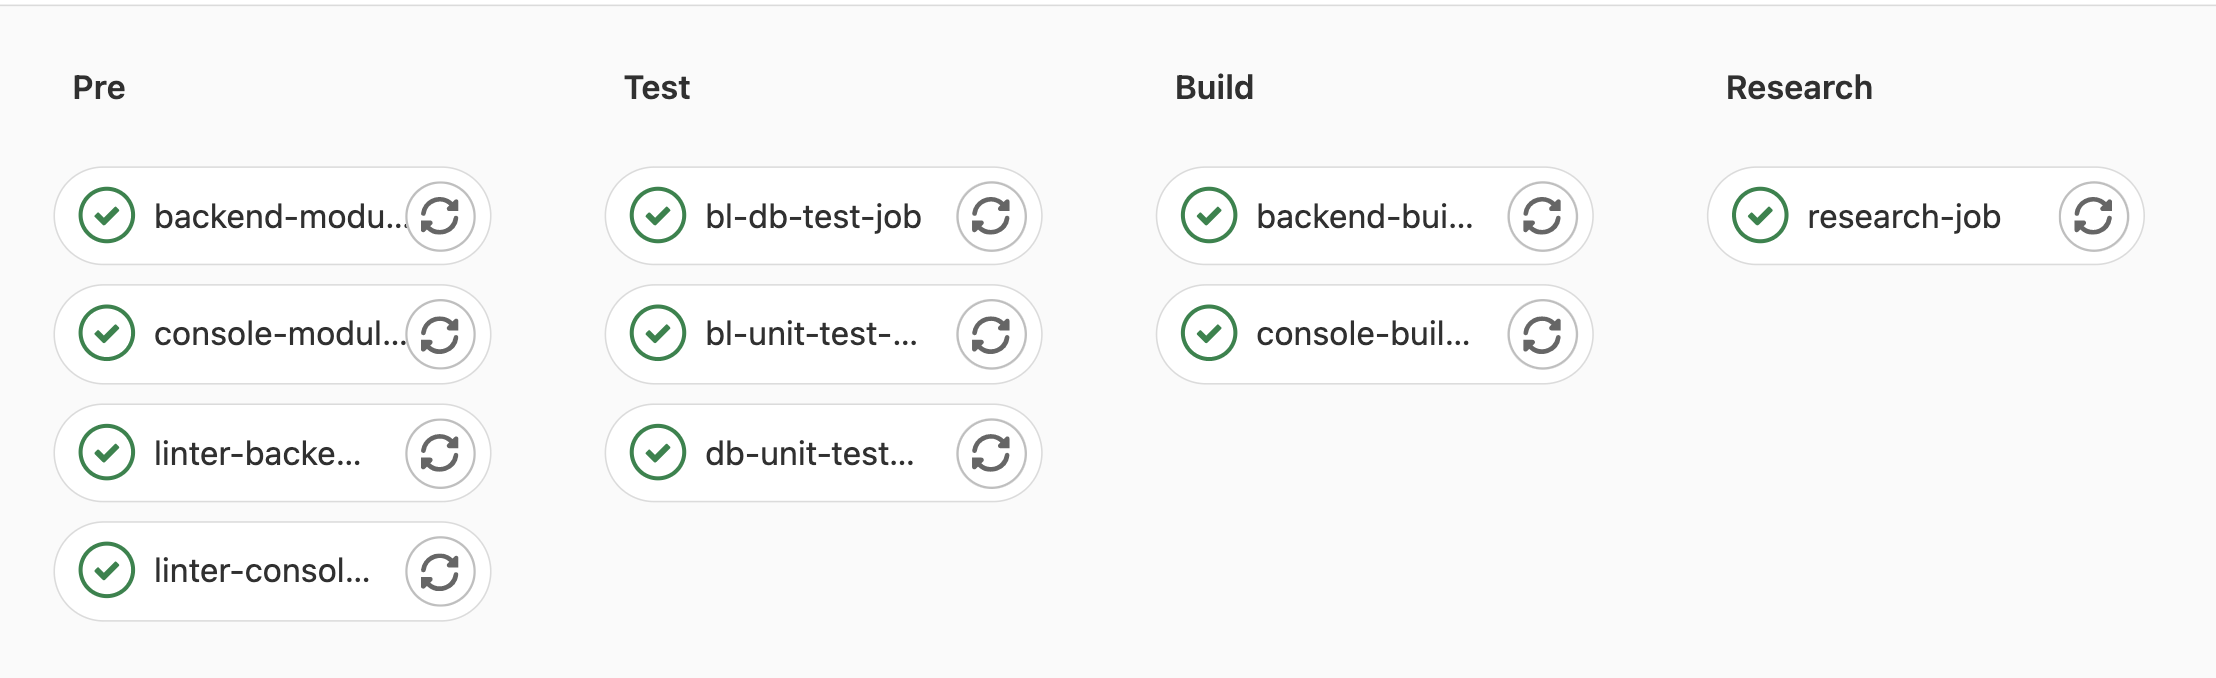
\includegraphics[width=\textwidth]{image/stages}
	\caption{Стадии сборочной линии}
	\label{stages}
\end{figure}

\begin{figure}[!h]
	\centering
	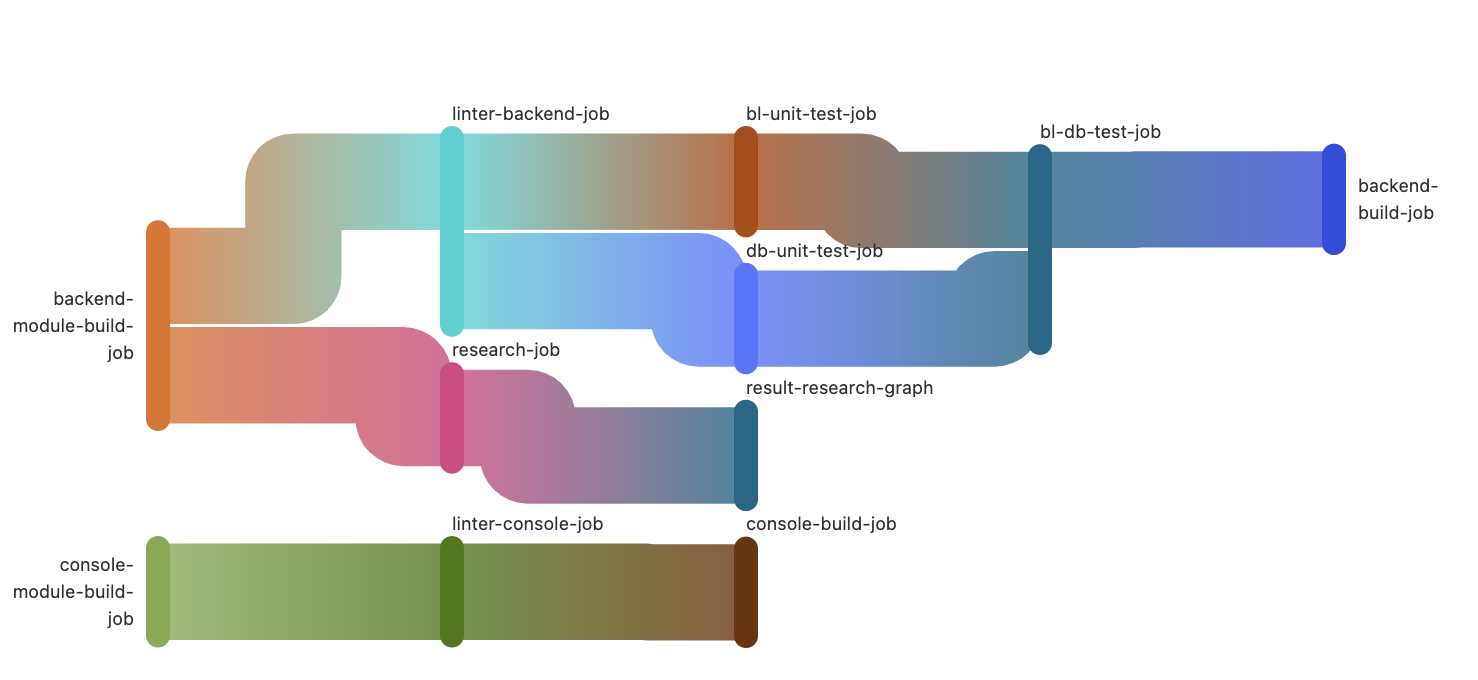
\includegraphics[width=\textwidth]{image/needs}
	\caption{Зависимости между заданиями}
	\label{needs}
\end{figure}




